%% LaTeX Beamer presentation template (requires beamer package)
%% see http://latex-beamer.sourceforge.net/
%% idea contributed by H. Turgut Uyar
%% template based on a template by Till Tantau
%% this template is still evolving - it might differ in future releases!

\documentclass{beamer}
\usepackage[utf8]{inputenc}
\usepackage{etex}

\mode<presentation>
{
\usetheme{Boadilla}
%\usetheme{Dresden}
%\usetheme{Madrid}
%\usetheme{Singapore}

\usecolortheme{wolverine}
%\usecolortheme{crane}
%\usecolortheme{dove}
%\usecolortheme{seagull}
%\usecolortheme{seahorse}
%\usecolortheme{rose}

\setbeamerfont{title}{shape=\itshape,family=\rmfamily}
%\setbeamercolor{title}{fg=red!80!black}
%\setbeamercolor{title}{fg=red!80!black,bg=red!20!white}

\usefonttheme{serif}
%\usefonttheme{structuresmallcapsserif}

\setbeamercovered{transparent}
}


\usepackage[english]{babel}
\usepackage{babelbib}

% font definitions, try \usepackage{ae} instead of the following
% three lines if you don't like this look
\usepackage{mathptmx}
\usepackage[scaled=.90]{helvet}
\usepackage{courier}


\usepackage[T1]{fontenc}
\usepackage{pictex}
\usepackage{dsfont}
\usepackage{ulem}


\title{ESE CPCC Project}

%\subtitle{}

% - Use the \inst{?} command only if the authors have different
%   affiliation.
%\author{F.~Author\inst{1} \and S.~Another\inst{2}}
\author{M. Kleber, C. Krainer, A. Schr\"ocker, B. Zechmeister}

% - Use the \inst command only if there are several affiliations.
% - Keep it simple, no one is interested in your street address.
\institute[University of Salzburg]
{
% \inst{1}%
Department of Computer Sciences\\
  University of Salzburg, Austria
% \and
% \inst{2}%
% Department of Theoretical Philosophy\\
% Univ of E
}

\date{\today}


% This is only inserted into the PDF information catalog. Can be left
% out.
\subject{Talks}



% If you have a file called "university-logo-filename.xxx", where xxx
% is a graphic format that can be processed by latex or pdflatex,
% resp., then you can add a logo as follows:

% \pgfdeclareimage[height=0.5cm]{university-logo}{university-logo-filename}
% \logo{\pgfuseimage{university-logo}}



% Delete this, if you do not want the table of contents to pop up at
% the beginning of each subsection:
\AtBeginSubsection[]
{
\begin{frame}<beamer>
	\frametitle{Outline}
	\tableofcontents[currentsection,currentsubsection]
\end{frame}
}

% If you wish to uncover everything in a step-wise fashion, uncomment
% the following command:

%\beamerdefaultoverlayspecification{<+->}

\begin{document}

\begin{frame}
	\titlepage
\end{frame}

\begin{frame}
	\frametitle{Content}
	\tableofcontents
% You might wish to add the option [pausesections]
\end{frame}


% - Einleitung
%   - Aufgabenstellung
%   - Systemarchitektur: Pilot, Engine, Mapper, GMView, Planner, ...
%   - Datenaustausch mit HTTP(S)
\section{Introduction}
%\subsection[Short First Subsection Name]{First Subsection Name}

\begin{frame}\frametitle{Introduction}\framesubtitle{Task}
	\begin{itemize}
		\item simulation of physical helicopter swarms
		\item simulation of sensors
		\item abstraction of virtual vehicles (virtual helicopters)
		\item migration of virtual vehicles among flying physical helicopters
	\end{itemize} 
\end{frame}

\begin{frame}\frametitle{Introduction}\framesubtitle{Project Scope}
	\begin{itemize}
		\item real vehicles (physical helicopters) follow strict flight plans
		\item no network bandwith limits
		\item no processing power limits
	\end{itemize} 
\end{frame}

\begin{frame}\frametitle{Introduction}\framesubtitle{Applied Technologies}
	\begin{itemize}
		\item HTTP as protocol for sensor abstraction and data exchange
		\item Java as programming language
		\item software implemented as web applications
		\item Apache Tomcat as web server and servlet container
	\end{itemize} 
\end{frame}

\begin{frame}\frametitle{Introduction}\framesubtitle{System Overview}
	{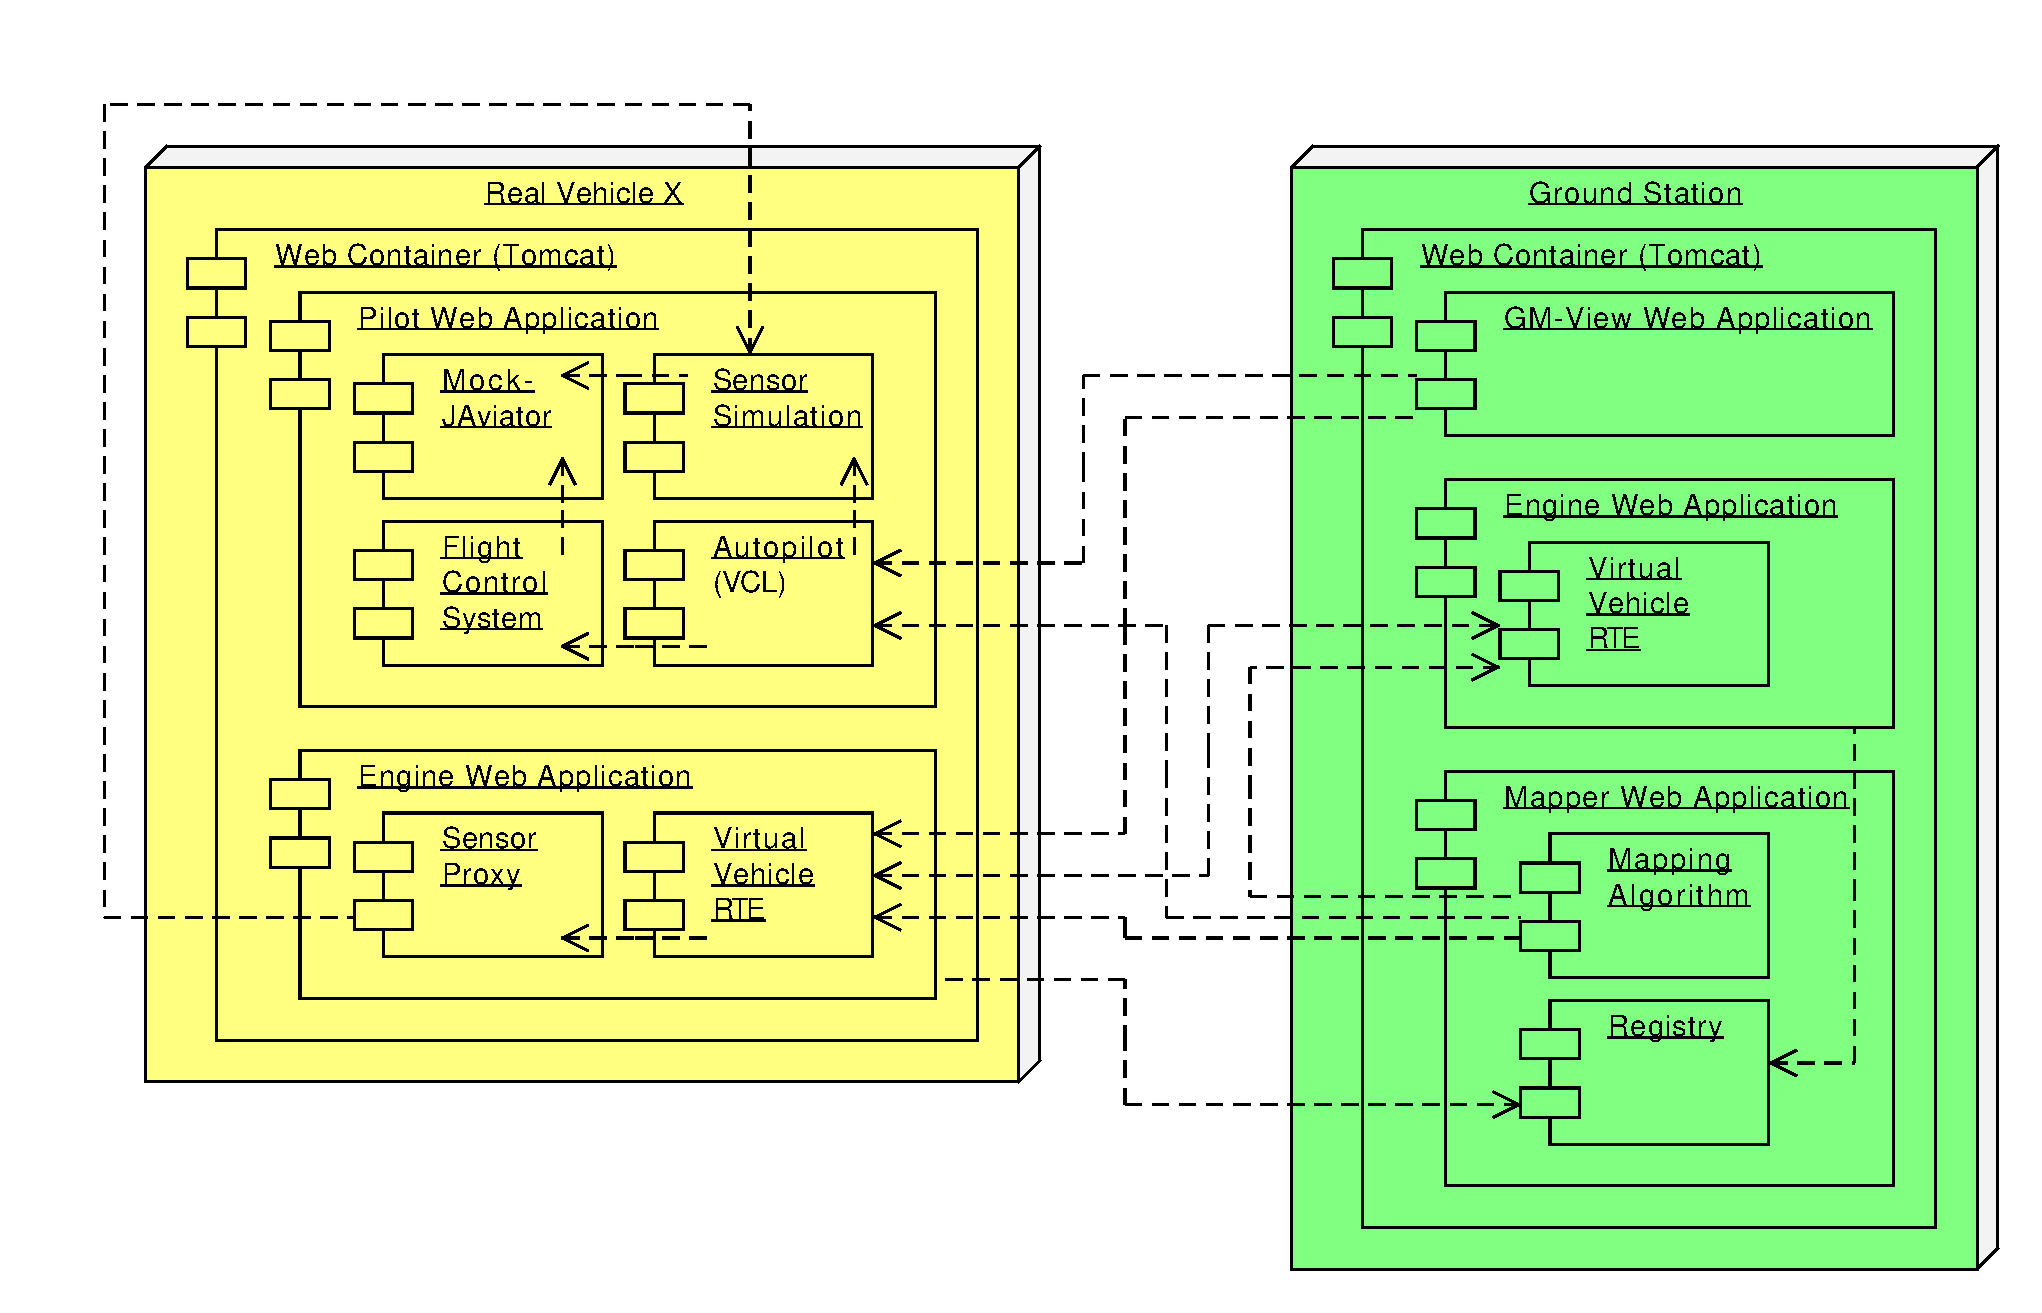
\includegraphics[width=11.5cm]{SystemOverview.pdf}}
\end{frame}

\begin{frame}\frametitle{Introduction}\framesubtitle{Sensor Simulation}
	{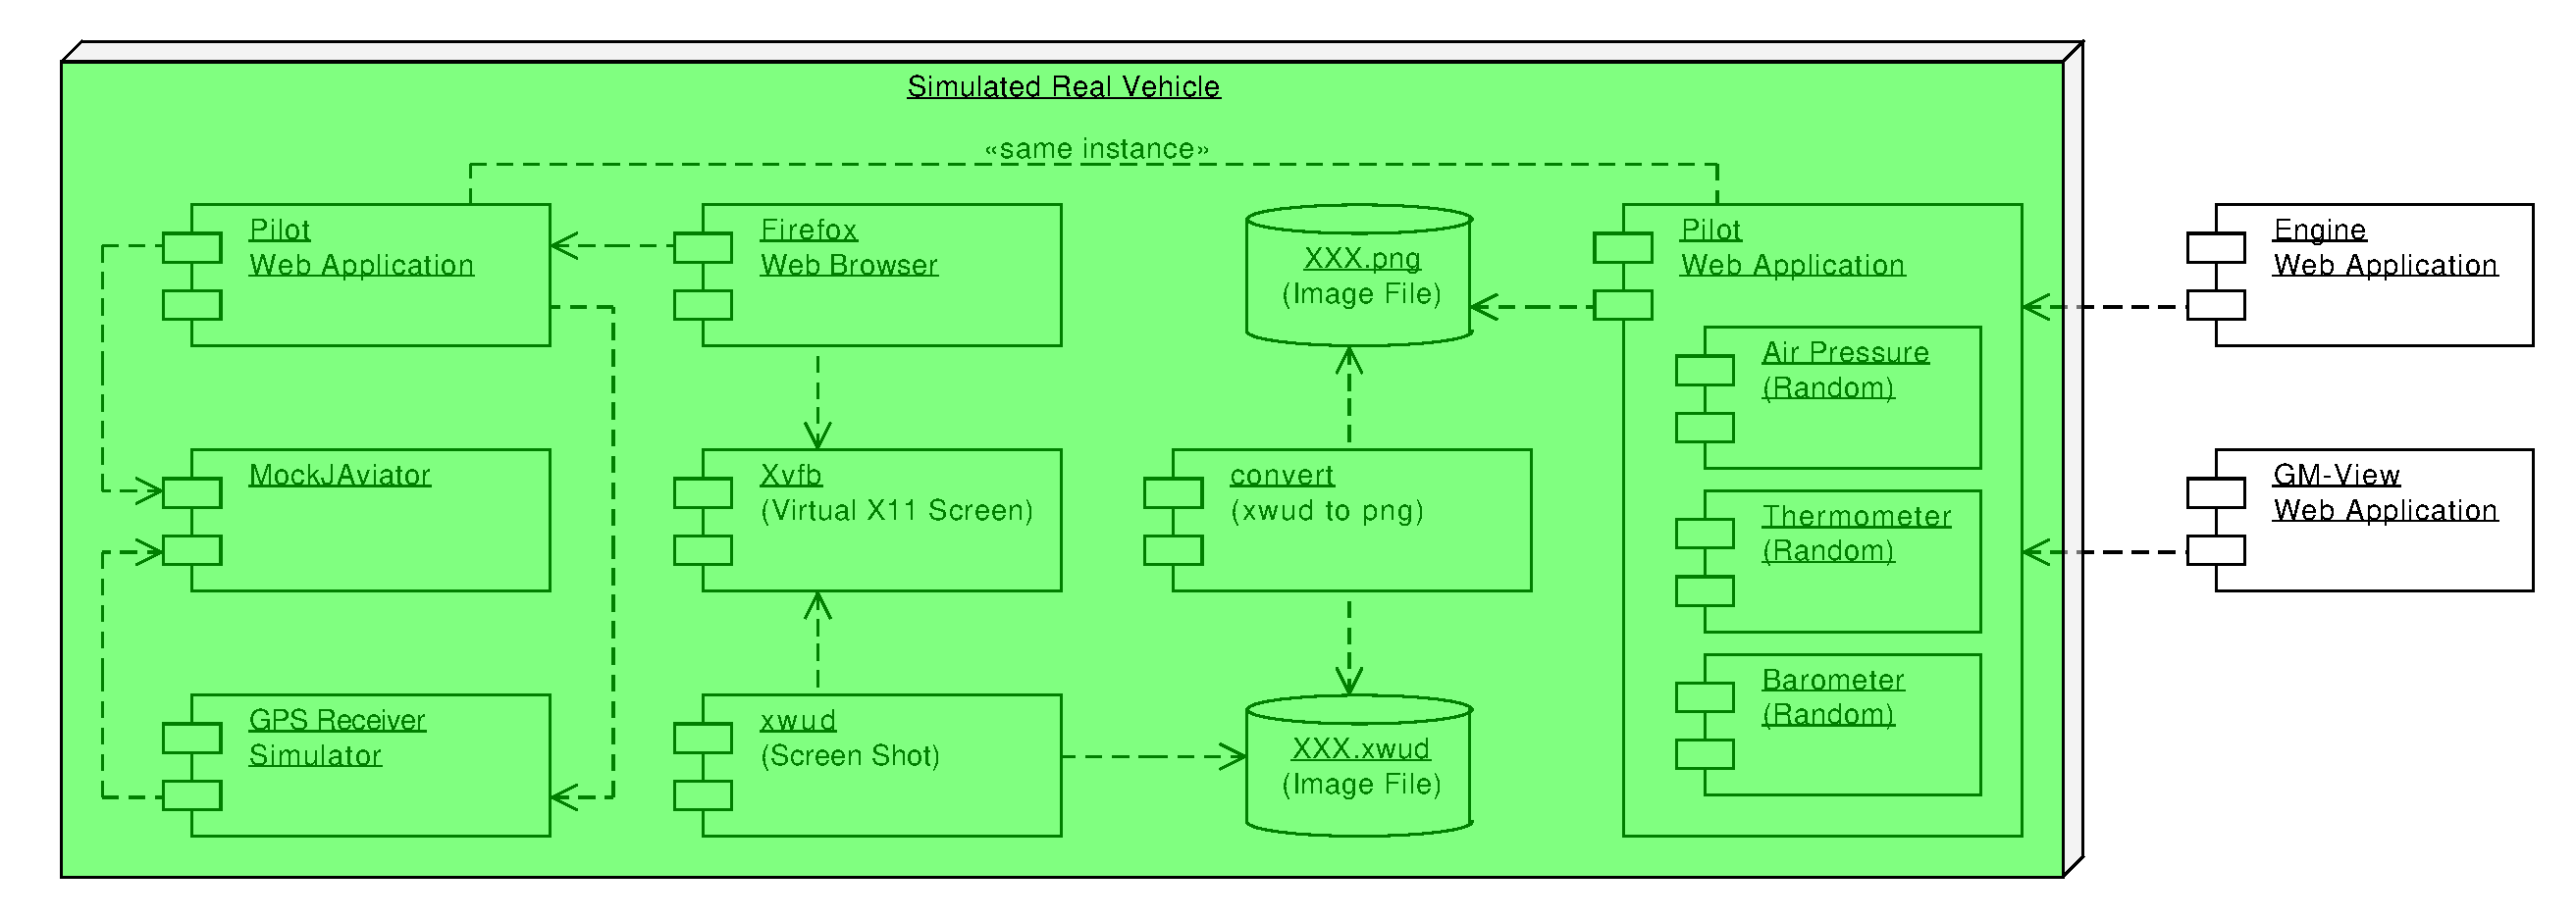
\includegraphics[width=11.5cm]{SensorSimulation.pdf}}
\end{frame}

% - Real Vehicles
%   - Flugplan / VCL
%   - Simulation
%   - Sensoren
\section{Real Vehicles}

\begin{frame}\frametitle{Sensor Simulation} %\framesubtitle{xxx}
	\begin{itemize}
		\item \ldots
		\item \ldots
	\end{itemize} 
\end{frame}

\begin{frame}\frametitle{Flight Plan} %\framesubtitle{xxx}
	\begin{itemize}
		\item real vehicles follow strict flight plans
		\item \ldots
	\end{itemize} 
\end{frame}




% - Vehicle Virtualisierung
%   - Prinzipielle Funktion eines VV-Programms
%   - Status / Serialisierung / Migration
%   - VV-Language: Command = Point + Actions
%   - Scanner, Parser
\section{Vehicle Virtualization}

\begin{frame}\frametitle{Virtual Vehicle Program} %\framesubtitle{xxx}
\begin{itemize}
\item ability to suspend
\item state is serialized
\item information is persisted to file
\item migration can be performed
\item virtual vehicle can resume
\end{itemize} 
\end{frame}

\begin{frame}\frametitle{Virtual Vehicle Language} %\framesubtitle{xxx}
\begin{itemize}
\item list of commands
\item command consits of a point and a list of actions
\item point contains latitude, longitude, altitude
\item specification of tolerance
\end{itemize} 
\end{frame}

\begin{frame}\frametitle{Virtual Vehicle Sample Program} %\framesubtitle{xxx}
\texttt{\\
Point 47.82201946 13.04082647 1.00 tolerance 12.3\\
Picture \\
Temperature\\
\\
Point 47.82203026 13.04084659 25.00 tolerance 100 \\
Temperature\\
\\
Point 47.82211311 13.04076076 30.00 tolerance 1.2\\
Picture} 
\end{frame}

\begin{frame}\frametitle{Scanner \& Parser} %\framesubtitle{xxx}
\begin{itemize}
\item \ldots
\end{itemize} 
\end{frame}

% - Mapping
%   - Registrierung der Engines
%   - Algorithmen: Random, Simple
%   - Ansto� der Migration
\section{Mapping}

\begin{frame}\frametitle{Engine Registration} %\framesubtitle{xxx}
\begin{itemize}
\item \ldots
\end{itemize} 
\end{frame}

% - Erk�rung User-Interface:
%   - GM-View
\section{User Interface}

\begin{frame}\frametitle{Google Maps Viewer} %\framesubtitle{xxx}
\begin{itemize}
\item \ldots
\end{itemize} 
\end{frame}


\section{Live Demonstration}
% - Demo 1: "VV sammelt Daten"
%   - Setup: 1xRV, 1xVV, 2xVV-Points
%   - RV fliegt die VV-Points ab
%   - VV sammelt die Daten ein
%\subsection{Demo 1 - Data Collection}

\begin{frame}\frametitle{Data Collection} %\framesubtitle{xxx}
\begin{itemize}
\item \ldots
\end{itemize} 
\end{frame}

% - Demo 2: "VV wird migriert"
%   - Setup: 2xRV, 1xVV, 2xVV-Points
%   - Je ein RV fliegt einen VV-Point an
%   - VV sammelt am RV1 die ersten VV-Point Daten
%     ein, wird migriert und macht am RV2 weiter.
%\subsection{Demo 2 - Migration}

\begin{frame}\frametitle{Virtual Vehicle Migration} %\framesubtitle{xxx}
\begin{itemize}
\item \ldots
\end{itemize} 
\end{frame}

% - Demo 3: "RVs haben unterschiedliche Sensoren"
%   - Setup: 3xRV, 1xVV, 1xVV-Point
%   - Alle RVs fliegen nacheinander einen VV-Point an
%   - VV sammelt am RV1 die ersten VV-Point Daten
%     ein, wird migriert auf RV2, sammelt weiter Daten
%     ein, wird migriert auf RV3 und sammelt die
%     restlichen Daten ein.
%\subsection{Demo 3 - Sensor Variety}

\begin{frame}\frametitle{Real Vehicles with different Sensors} %\framesubtitle{xxx}
\begin{itemize}
\item \ldots
\end{itemize} 
\end{frame}


% - Demo 4: "All in one."
%   - Setup: 3xRV, 3xVV, 9xVV-Point
%   - ...
%\subsection{Demo 4 - All in One}

\begin{frame}\frametitle{All in One} %\framesubtitle{xxx}
\begin{itemize}
\item \ldots
\end{itemize} 
\end{frame}

% - Future Work
%   - Aufw�ndigere Mapping-Algorithmen
%   - Optimierung Netzwerkverkehr
%   - Video-Sensor
%   - Geo-Location: Vergleich RV-Position zu VV-Sollwert
%   - RV-Flugpl�ne aus VV-Programmen zusammenstellen
\section{Future Work}

\begin{frame}\frametitle{Future Work} %\framesubtitle{xxx}
	\begin{itemize}
		\item more sophisticated mapping algorithms
		\item network traffic optimizations
		\item video sensor support
		\item extended geo-location
		\item flight plan generation
	\end{itemize}
\end{frame}
 

% - Q & A Session
\section{Questions and Answers}

\begin{frame}
	\frametitle<presentation>{Questions \& Answers}
	\framesubtitle{~}
	\begin{center}
		\fontsize{64}{64}\selectfont
		\begin{tabular}{ccc}
			Q &&\\
			& ~~\& & \\
			&&~~ A
		\end{tabular}
	\end{center}
\end{frame}

% Sample Frame:
% \begin{frame}
% \frametitle{Introduction}
% %\framesubtitle{xxx}
% 
% Test $\displaystyle{x = (x_n)_{n\in\mathds{N}_0}}$
% 
% Test
% \begin{equation}
% 	x : \mathds{N}_0 \rightarrow \mathds{C}
% \end{equation}
% 
% \pause
% 
% Test
% \begin{equation}
% 	\mathcal{Z}\{x\} =
% 	X(z) := \sum_{n=0}^\infty x_n\cdot z^{-n} ~, \qquad z\in \mathds{C}
% \end{equation}
% 
% \pause
% \vspace{0.5cm}
% $\displaystyle{X(z)}$ ist f\"ur die $\displaystyle{z\in\mathds{C}}$ definiert, f\"ur die die
% unendliche Reihe konvergiert.
% 
% %$\displaystyle{\sum_{k=0}^\infty x_k\cdot z^{-k}}$ konvergent ist.
% 
% \end{frame}

\end{document}
